% !TEX TS-program = LuaLaTeX
\documentclass[11pt,compress,xcolor=x11names,UTF8]{beamer}
\usetheme{Boadilla}
\usecolortheme{seahorse}
\useinnertheme[shadow]{rounded}  
\useoutertheme[subsection=false]{smoothbars}
\usecolortheme{spruce}
\usecolortheme[named=SpringGreen4]{structure}
\usefonttheme{structurebold}
\useinnertheme{circles}
\usecolortheme{rose}
\usepackage{pifont}
\usepackage{academicons}
\usepackage{fontawesome}
\usepackage{iitem}
\usepackage{graphicx}
\usepackage{tabularx}
\usepackage{amsmath,amssymb}
\DeclareMathOperator*{\SIGMA}{SIGMA}
\setbeamertemplate{itemize item}{\ding{108}}
\setbeamertemplate{itemize subitem}{\ding{109}}
\setbeamertemplate{navigation symbols}{}
\setbeamercovered{transparent}  
\renewcommand\appendixname{附录}
\renewcommand\abstractname{摘要}
\graphicspath{{figure/}} % 图片路径
\usepackage{calligra} % Thank you
\usepackage{ctex} % 加入中文
%\setCJKsansfont{Noto Sans CJK SC}
\setsansfont{Lato} % Lato Roboto Fira Sans
\usepackage{makecell}
\newcommand{\tabincell}[2]{\begin{tabular}{@{}#1@{}}#2\end{tabular}}
\usepackage{url}					
\usepackage{natbib} % 参考文献
%\title[Spatial Generalized Linear Mixed Models]{Spatial Generalized Linear Mixed Models with Application to Prevalence Mapping}
%\title{江门中微子实验与小型反应堆中微子探测器}
\title{江门中微子实验近点探测器研究}
\subtitle{开题报告}
\author[赵荣]{Email:zhaor25@mail2.sysu.edu.cn \and  } % \\ 专业:统计学 \\ 方向:数据分析与统计计算
\institute[中山大学]{School of Physics\and } % 理学院\\
\date[\today]{
\includegraphics[width=.5\textwidth]{logo}}

\begin{document}

\maketitle

\begin{frame}{Outline}
\tableofcontents
\end{frame}

\section{背景简介}

%\subsection{研究意义}

\begin{frame}{江门中微子实验}
%\textsf{例} \textbf{例}  \textit{例} 
% \texttt{例}  % 调出仿宋字体了

江门中微子实验(JUNO)是一个精确测量反应堆中微子的能谱的实验,主要物理目标是确定中微子的质量顺序\footnote{Neutrino Physics with JUNO - JUNO Collaboration (An, Fengpeng et al.) J.Phys. G43 (2016) no.3, 030401 arXiv:1507.05613 [physics.ins-det] }。
\begin{figure}
\centering
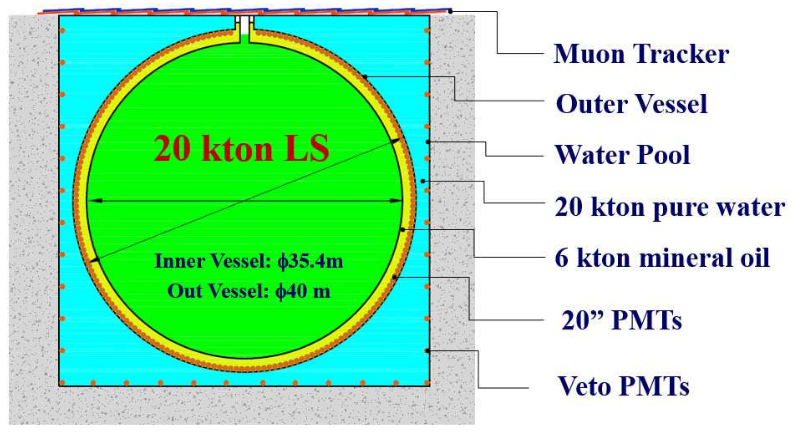
\includegraphics[width=.6\textwidth]{k_junodet} % 单图
\caption{JUNO的探测器示意图}
\end{figure}
\end{frame}
%%%%%%%%%%%%%%%%%%%%%%%%%%%%%%%%%%%%%%%%%%%
\begin{frame}{江门中微子实验}
JUNO属于中基线反应堆中微子实验,基线长度53Km,设计能量分辨率3\%/$\sqrt{E(\text{MeV})}$。
\begin{figure}
\centering
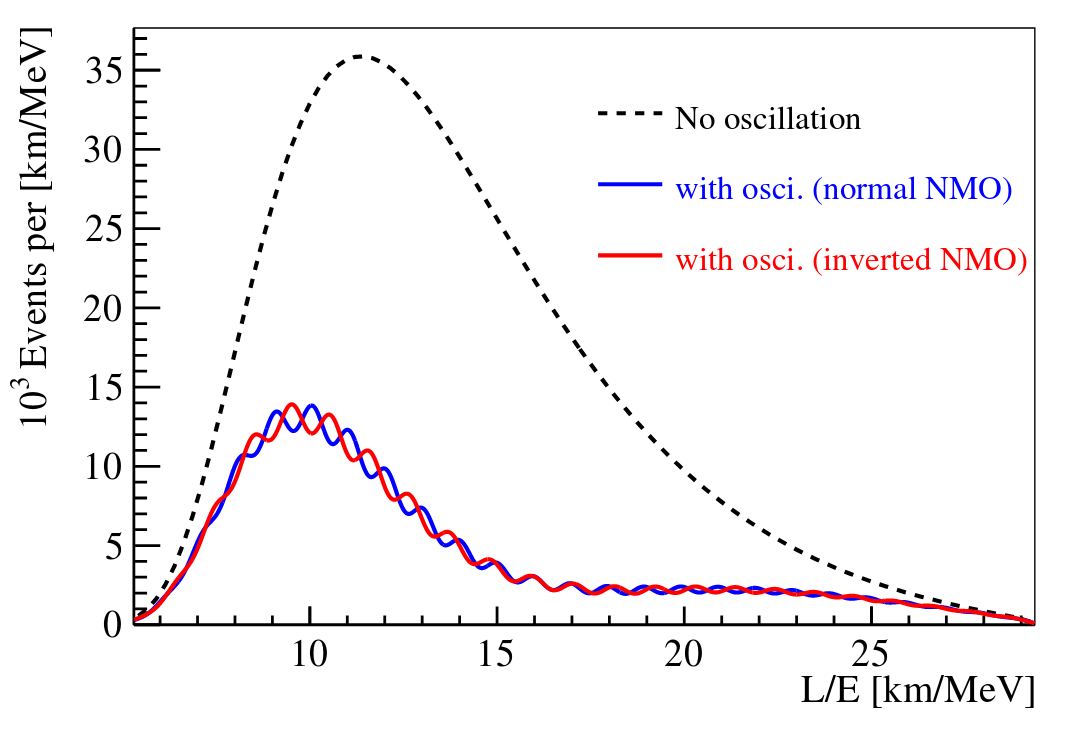
\includegraphics[width=0.58\textwidth]{k_nuosi} % 单图
\caption{不同质量顺序下的JUNO反应堆能谱}
\end{figure}
\end{frame}
%%%%%%%%%%%%%%%%%%%%%%%%%%%%%%%%%%%%%%%%%%%
\begin{frame}{IBD事件}
\begin{columns}
\begin{column}{.5\textwidth}
\begin{figure}
\centering
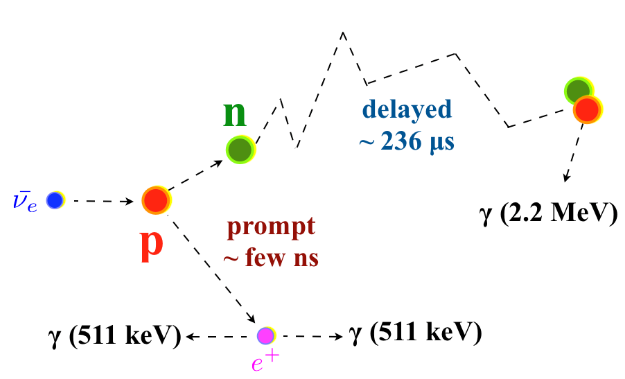
\includegraphics[width=\textwidth]{k_IBDevt} % 单图
\caption{IBD事件的探测原理}
\end{figure}
\end{column}
\begin{column}{.45\textwidth}
JUNO间接中微子:通过探测反$\beta$衰变产生的正电子以及中子来确定中微子的能谱。
\vspace{.5cm}
\hrule{\textwidth}
\vspace{.5cm}

\alert{正电子信号和俘获中子信号的事件符合,可以减少实验的本底}

\vspace{.5cm}
\hrule{\textwidth}
\vspace{.5cm}
实验上的可测量物理量是正电子的能量$E_{vis}$($E_{e^+}$)
\begin{equation}
E_{vis}=E_{\nu}-0.8\text{MeV}
\end{equation}
\end{column}
\end{columns}
\end{frame}
%%%%%%%%%%%%%%%%%%%%%%%%%%%%%%%%%%%%%%%%%%%
%~~!!!!!!!!!!!!!!!!!!put two figures to illustrate!!!!!
\begin{frame}{反电子中微子的能谱}
\begin{columns}
\begin{column}{.5\textwidth}
\begin{figure}
\centering
\includegraphics[width=\textwidth]{K_ibdspec} % 单图
\caption{反应堆中微子$\bar{\nu_e}$}的能谱
\end{figure}
\end{column}
\begin{column}{.45\textwidth}
反应堆中四种同位素裂变产生中微子,传播一段时间之后被探测器探测到。
\[
\Phi(E_{\nu})=\frac{W_{th}}{\Sigma_{i} f_{i}e_{i}}\cdot\Sigma\limits_{i} f_{i}\cdot S_{i}(E_{\nu})
\]
\vspace{.1cm}

\hrule{\textwidth}
\vspace{.5cm}
为了准确预测探测器的中微子能谱分布,需要精确计算反应堆{\color{blue}产生的中微子能谱},以及中微子在{\color{blue}传播过程中的振荡}。
\end{column}
\end{columns}
\end{frame}
%%%%%%%%%%%%%%%%%%%%%%%%%%%%%%%%%%%%%%%%%%%
\begin{frame}{反应堆中微子能谱理论和测量}
%安封彭,博士论文
\begin{figure}
\centering
\includegraphics[width=.8\textwidth]{K_rate} % 单图
\caption{反应堆中微子$\bar{\nu_e}$的事例率}
\end{figure}
反应堆能谱的细小结构带来的不确定性,会使得JUNO对质量顺序的分辨能力变弱\footnote{ arXiv:1710.07378}。
反应堆中多种产生中微子的过程比较复杂,目前模型对中微子的能谱预测的误差较大;需要准确测量各种中微子反应的参数来完善模型。
\end{frame}
%%%%%%%%%%%%%%%%%%%%%%%%%%%%%%%%%%%%%%%%%%%
\begin{frame}{反应堆中微子异常}
arxiv.org/pdf/1704.01082.pdf\qquad 
arxiv.org/pdf/1607.05378.pdf
%\vspace{-.8cm}
\begin{columns}
\begin{column}{.45\textwidth}
\begin{figure}
\centering
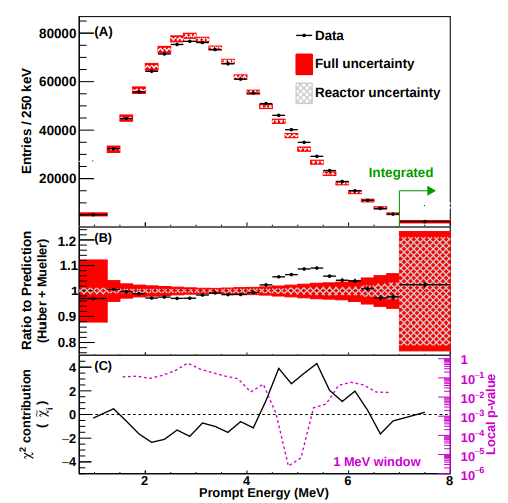
\includegraphics[width=\textwidth]{dybspe} % 单图
\caption{大亚湾中微子能谱}
\end{figure}
\end{column}
\begin{column}{.45\textwidth}
\begin{figure}
\centering
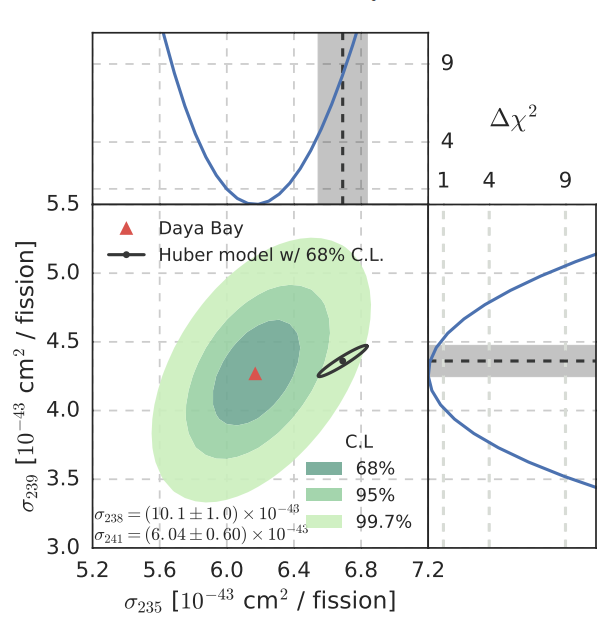
\includegraphics[width=\textwidth]{k_dayspe} % 单图
\caption{大亚湾中微子反应截面}
\end{figure}
\end{column}
\end{columns}

\end{frame}
%%%%%%%%%%%%%%%%%%%%%%%%%%%%%%%%%%%%%%%%%%%
\begin{frame}{反应堆中微子能谱}
arxiv:1511.05849 \qquad arxiv:1406.7763
\begin{columns}
\begin{column}{.4\textwidth}
\begin{figure}
\centering
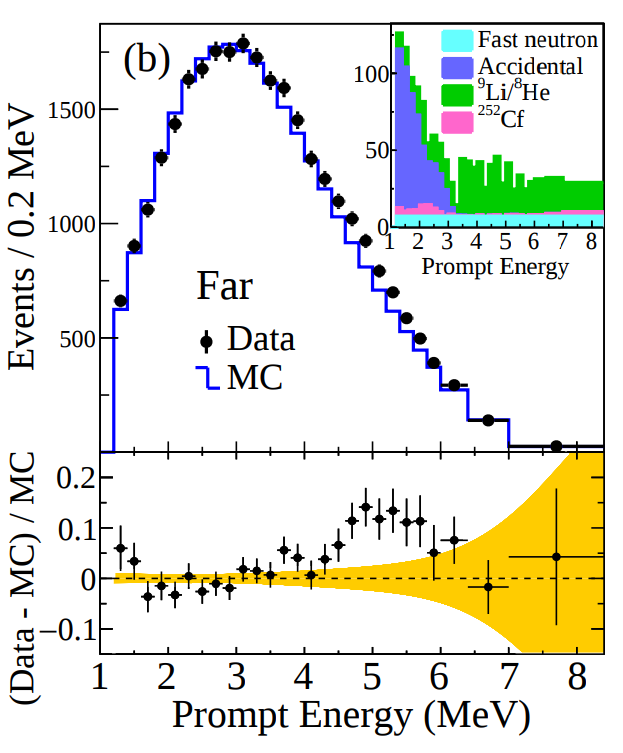
\includegraphics[width=\textwidth]{k_RENO} % 单图
\caption{RENO中微子能谱}
\end{figure}
\end{column}
\begin{column}{.45\textwidth}
\begin{figure}
\centering
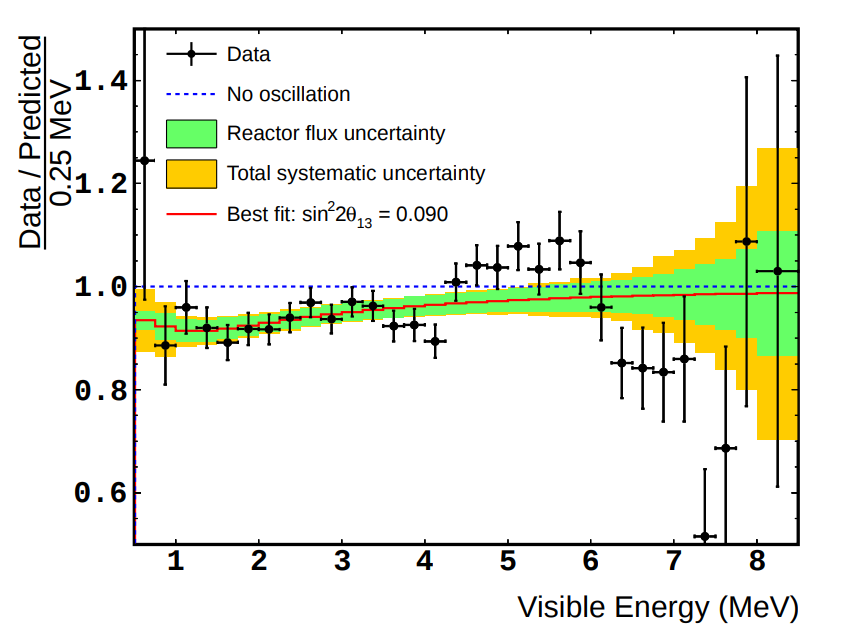
\includegraphics[width=\textwidth]{k_doublechooz} % 单图
\caption{Double Chooz}
\end{figure}
\end{column}
\end{columns}
\end{frame}
%%%%%%%%%%%%%%%%%%%%%%%%%%%%%%%%%%%%%%%%%%%%%%
\section{JUNO近点探测器-TAO}
%%%%%%%%%%%%%%%%%%%%%%%%%%%%%%%%%%%%%%%%%%%
\begin{frame}{Mtivation}
建立一个和JUNO主探测器类似的小型近点探测器,抵消关联误差,减小能谱测量不确定性对JUNO的影响。

已经通过JUNO合作组认可,命名Tai-shan Antineutrino Observatory.
\vspace{.1cm}

\hrule{\textwidth}
\vspace{.5cm}
IHEP 方案:液体闪烁体+SiPM.
其他方案:塑料闪烁体+SiPM(PMT).
\vspace{.1cm}

\hrule{\textwidth}
\vspace{.5cm}
目前国际上有多个反应堆监控的中微子探测器,相关的技术比较成熟,可以参考借鉴之前的经验。
\end{frame}
%%%%%%%%%%%%%%%%%%%%%%%%%%%%%%%%%%%%%%%%%%%
%\begin{frame}{液体闪烁体近点探测器方案}
%IHEP
%\end{frame}
%%%%%%%%%%%%%%%%%%%%%%%%%%%%%%%%%%%%%%%%%%%
\begin{frame}{塑料闪烁体方案}
探测原理:IBD,通过$e^+$和n的符合信号来鉴别中微子事件,MiniCHANDLER(http://www.aap.sympnp.org/Talks/Camillo.pdf).
\begin{figure}
\centering
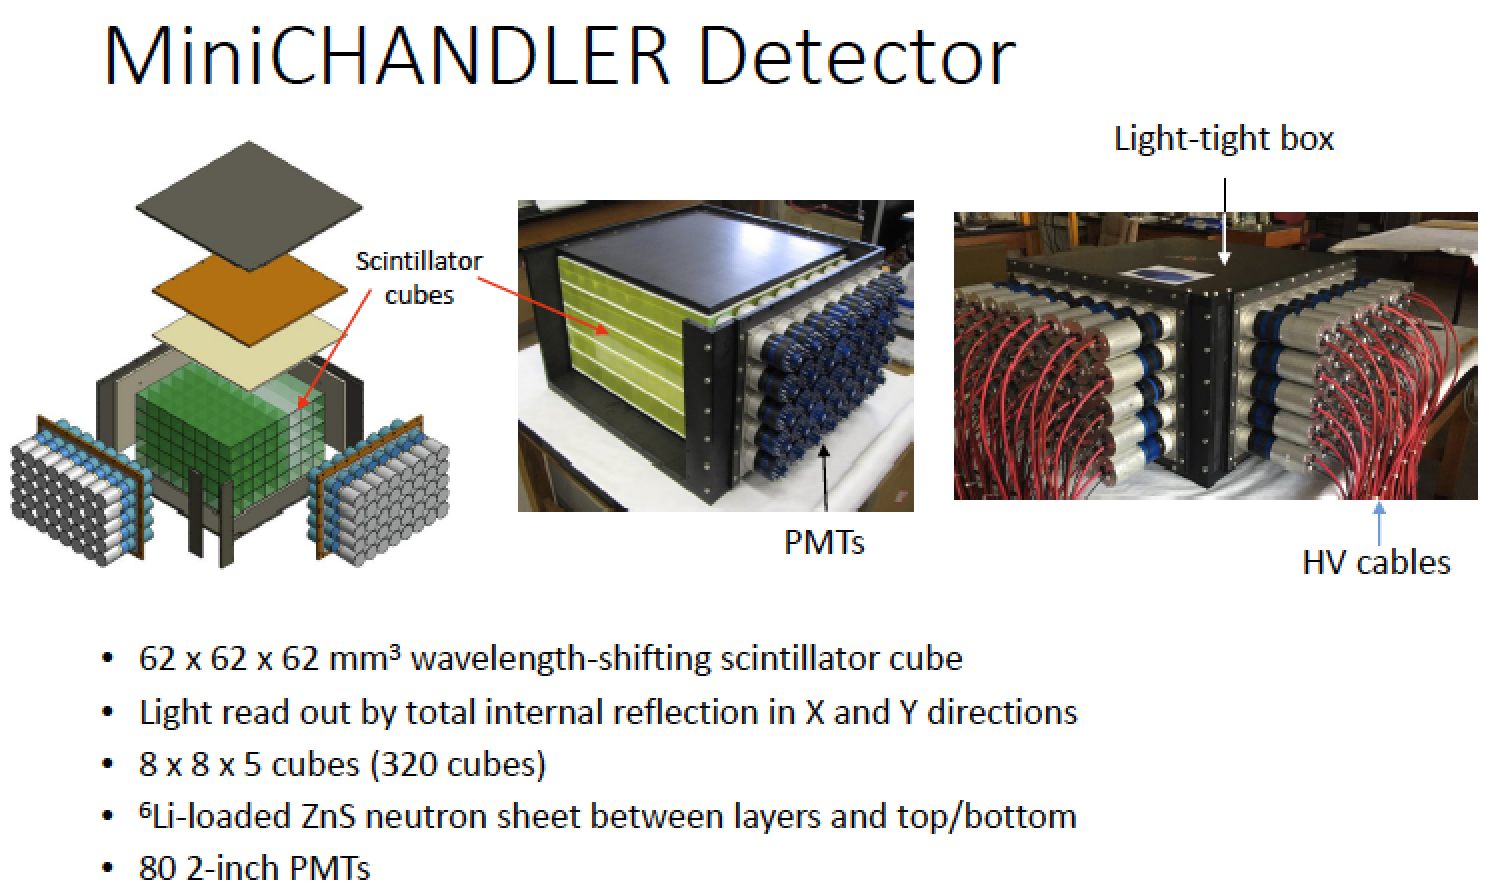
\includegraphics[width=.869\textwidth]{hor} % 单图
\caption{MiniCHANDLER}
\end{figure}
\end{frame}

%%%%%%%%%%%%%%%%%%%%%%%%%%%%%%%%%%%%%%%%%%%
%~~!!!!!!!!!!!!!!!!!!put two figures to illustrate!!!!!
%\begin{frame}{JUNO测量质量等级的灵敏度}
%\begin{columns}
%\begin{column}{.5\textwidth}
%\begin{figure}
%\centering
%\includegraphics[width=\textwidth]{K_msh} % 单图
%\end{figure}
%\begin{equation}
%\Delta\chi^2_{MH}=|\chi^2_{min}(N)-\chi^2_{min}(I)|
%\end{equation}
%
%\end{column}
%\begin{column}{.45\textwidth}
%101抽屉一直放置参考PMT EA0419,抽屉因子$drawer_{factor}$拟合的结果随着时间漂移,这存在两种可能:
%\vspace{.5cm}
%\hrule{\textwidth}
%\vspace{.5cm}
%\begin{itemize}
%\item 光源光强随时间变化(光强减小)
%\item PMT自身的性能PDE在减小
%\end{itemize}
%
%\end{column}
%\end{columns}
%\end{frame}
\section{探测器硬件以及模拟研究}
%%%%%%%%%%%%%%%%%%%%%%%%%%%%%%%%%%%%%%%%%%%
\begin{frame}{闪烁体性能测试}
闪烁体的基本性能测试:
\begin{itemize}
%\item 因为MCP和HAMAMATSU 两种PMT的性能差异较大,需要对两种PMT分别计算$f_{cs}$。
\item 光产额
\item 衰减长度
\item 发光时间
\item 发光光谱
\end{itemize}
\vspace{.5cm}
\hrule{\textwidth}
\vspace{.5cm}

选择PMT或者SiPM作为光子探测器,需要测试各种重要参数:
\begin{itemize}
\item 探测效率
\item 光子分辨率等
\item 工作条件和稳定性
\end{itemize}
\end{frame}
%%%%%%%%%%%%%%%%%%%%%%%%%%%%%%%%%%%%%%%%%%%
%%%%%%%%%%%%%%%%%%%%%%%%%%%%%%%%%%%%%%%%%%%
%\begin{frame}{光电转换器件性能测试}
%\begin{columns}
%\begin{column}{\textwidth}
%选择PMT或者SiPM作为光子探测器,需要测试各种重要参数:
%\begin{itemize}
%\item 探测效率
%\item 光子分辨率等
%\item 工作条件和稳定性
%\end{itemize}
%\begin{figure}
%\centering
%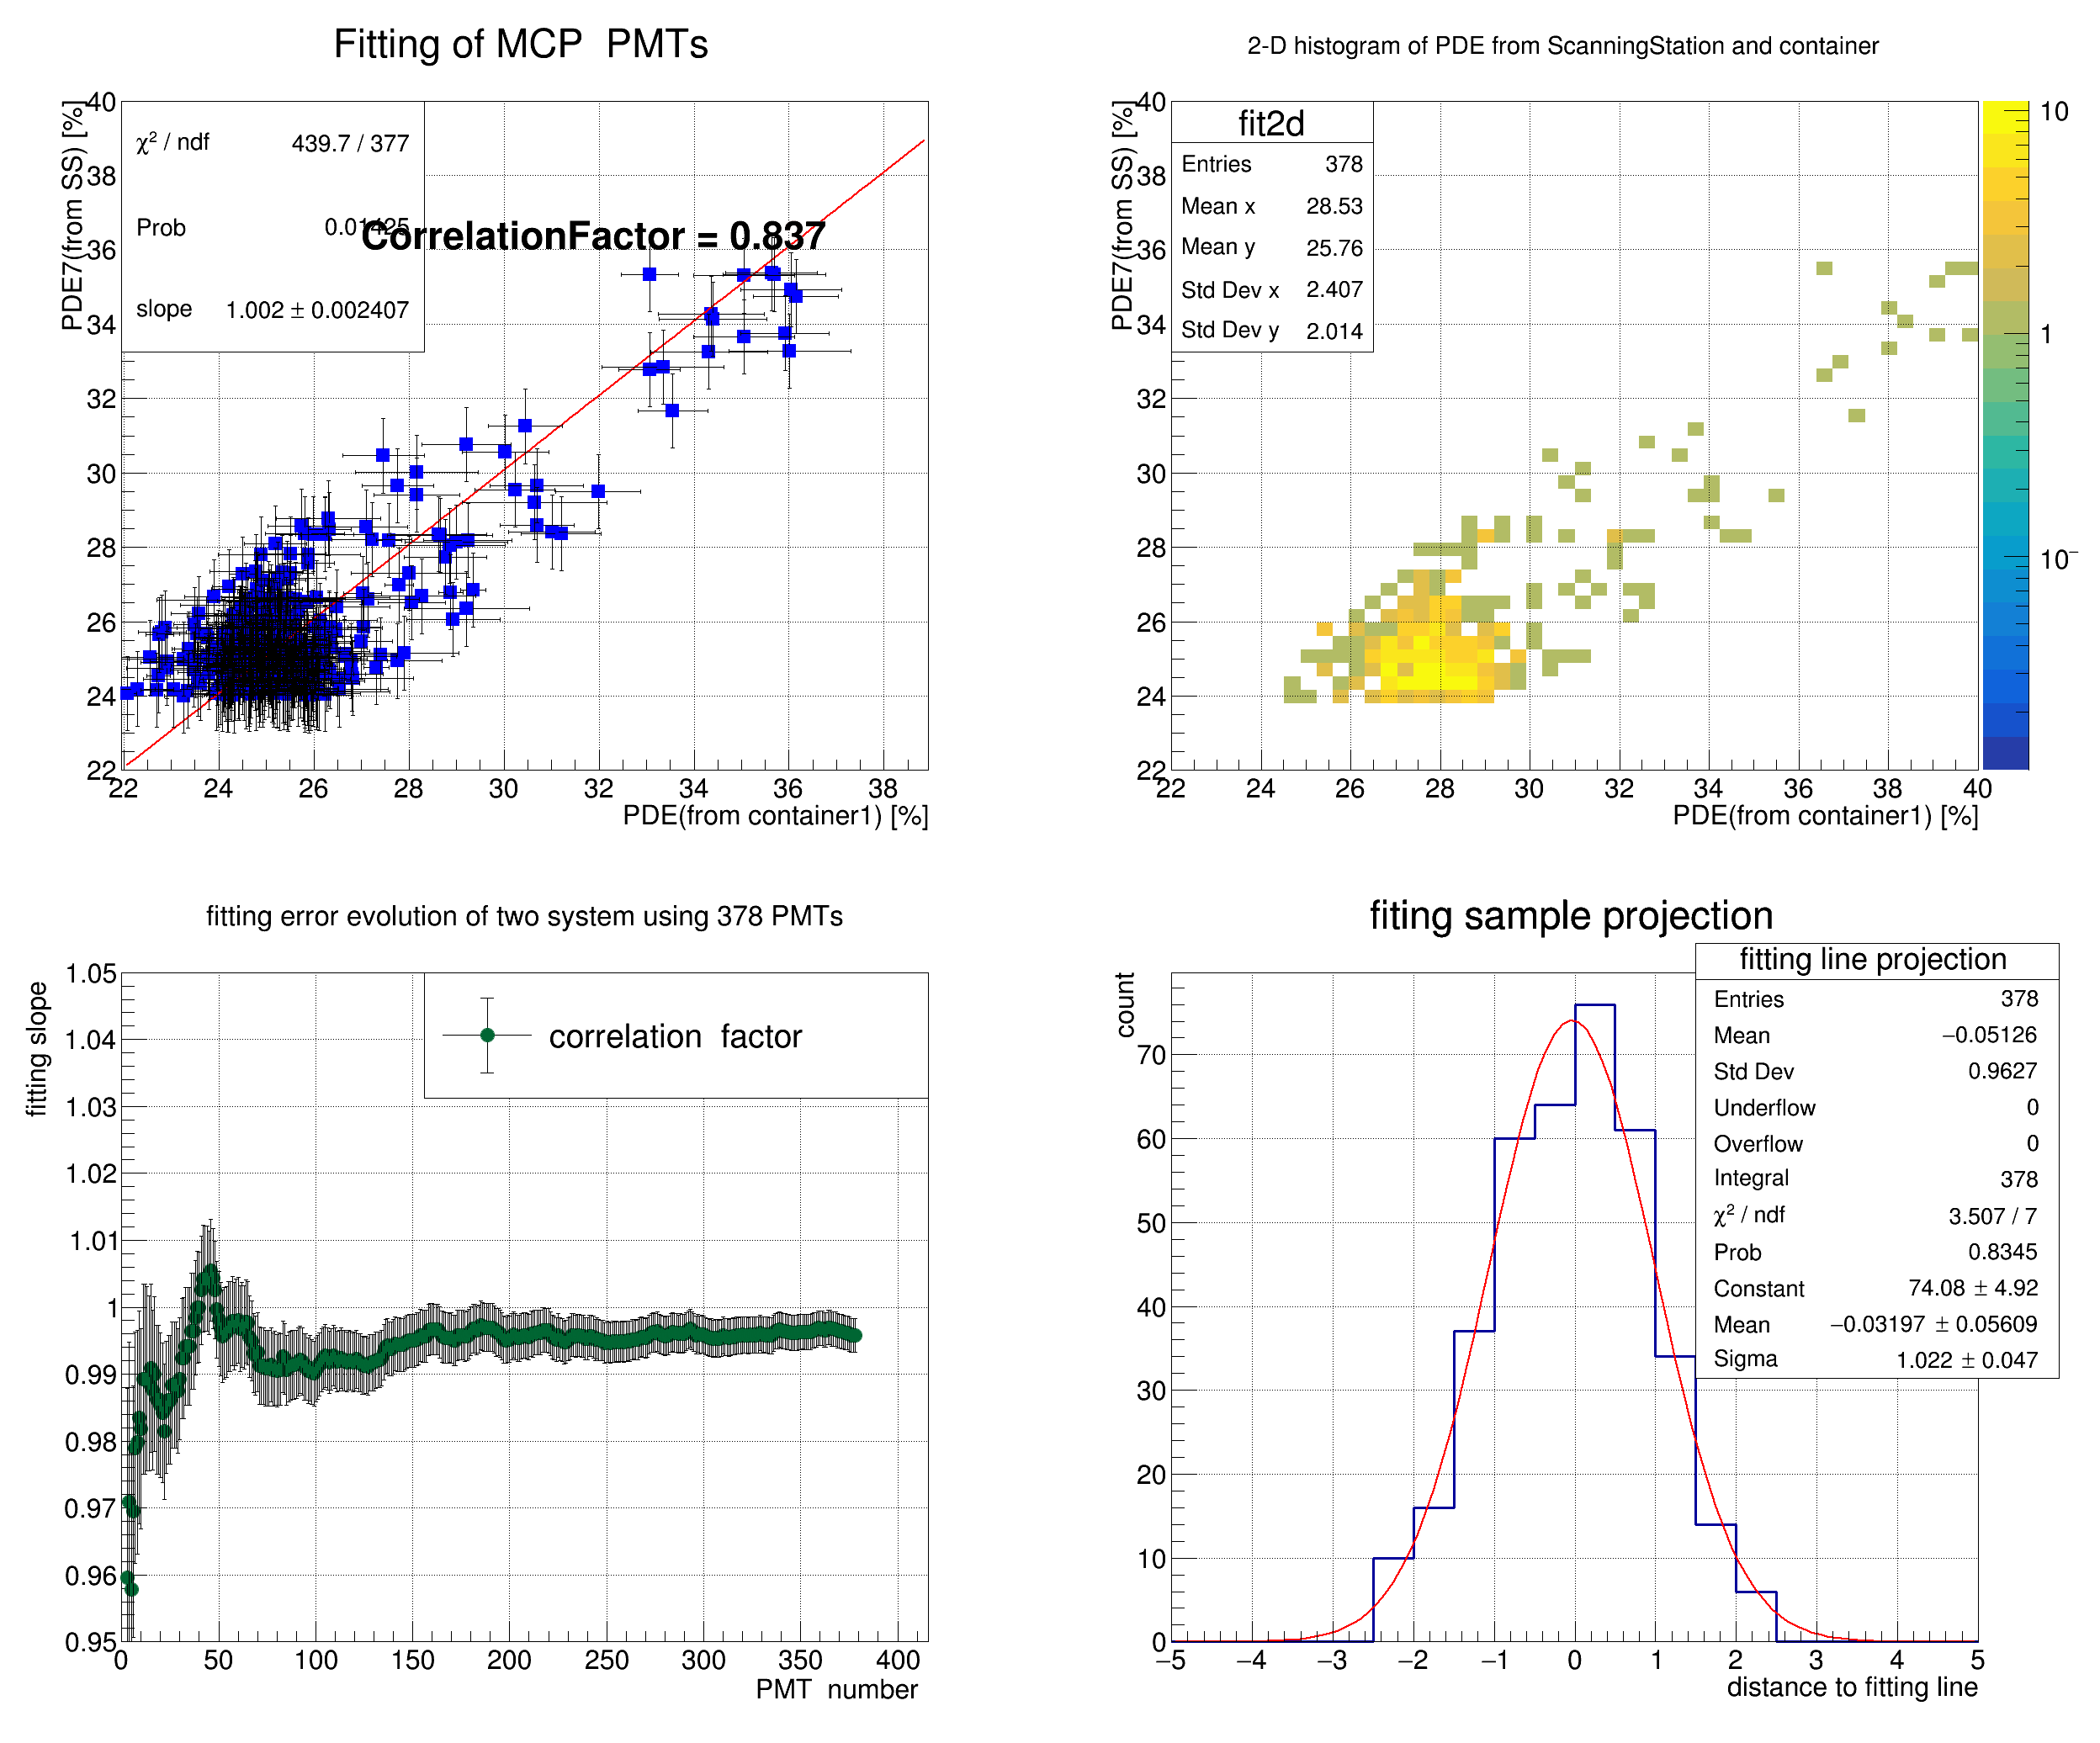
\includegraphics[width=0.58\textwidth]{fit_mcp_noint}
%\end{figure}
%\end{column}
%\begin{column}{.001\textwidth}

%\end{column}
%\end{columns}
%\end{frame}

%%%%%%%%%%%%%%%%%%%%%%%%%%%%%%%%%%%%%%%%%%%%%%%%%%%%%%%%%%%%%%%%%%%%
\begin{frame}{探测器设计和优化}
根据闪烁体和光电器件的测试结果和探测器模拟,对整个探测器几何结构以及参数选择进行优化。提高事例鉴别的准确率,减小本底信号。
\begin{itemize}
\item 如何鉴别闪烁体的输出信号是$\gamma$还是中子产生的?
\item 怎么样挑选中微子事例 
\item $\mu$ veto 以及如何屏蔽环境本底
\end{itemize}
\begin{figure}
\centering
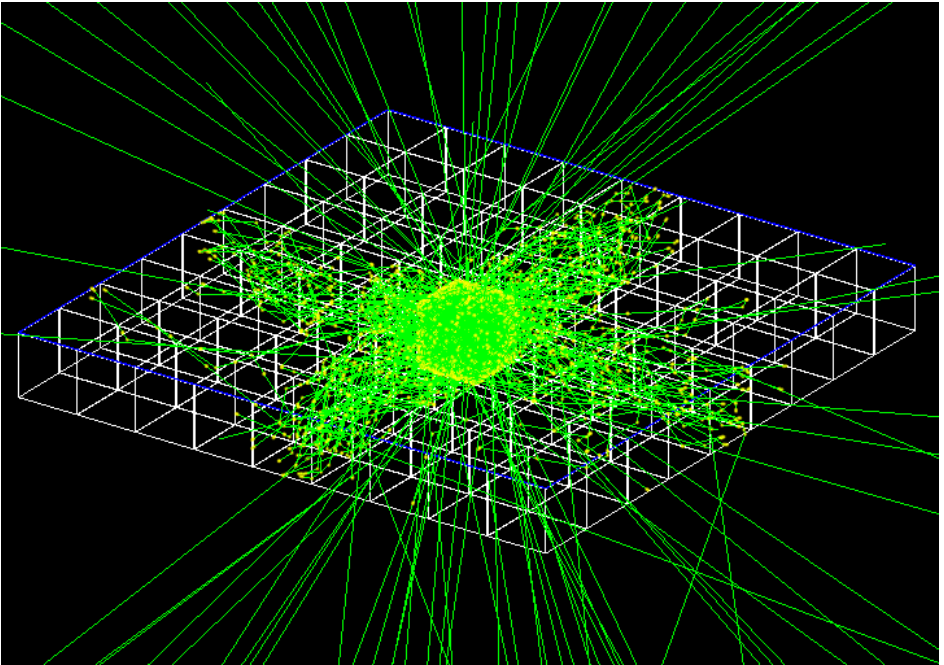
\includegraphics[width=.6\textwidth]{g4sim} % 单图
\caption{GEANT4 simulation}
\end{figure}
%利用$PDE_c$和$PDE_s$对所有HAMAMATSU-PMT拟合$f_{cs}$的结果\footnote{挑选条件:集装箱测试合格而且$\Delta PDE<5$}:
%\begin{figure}
%\centering
%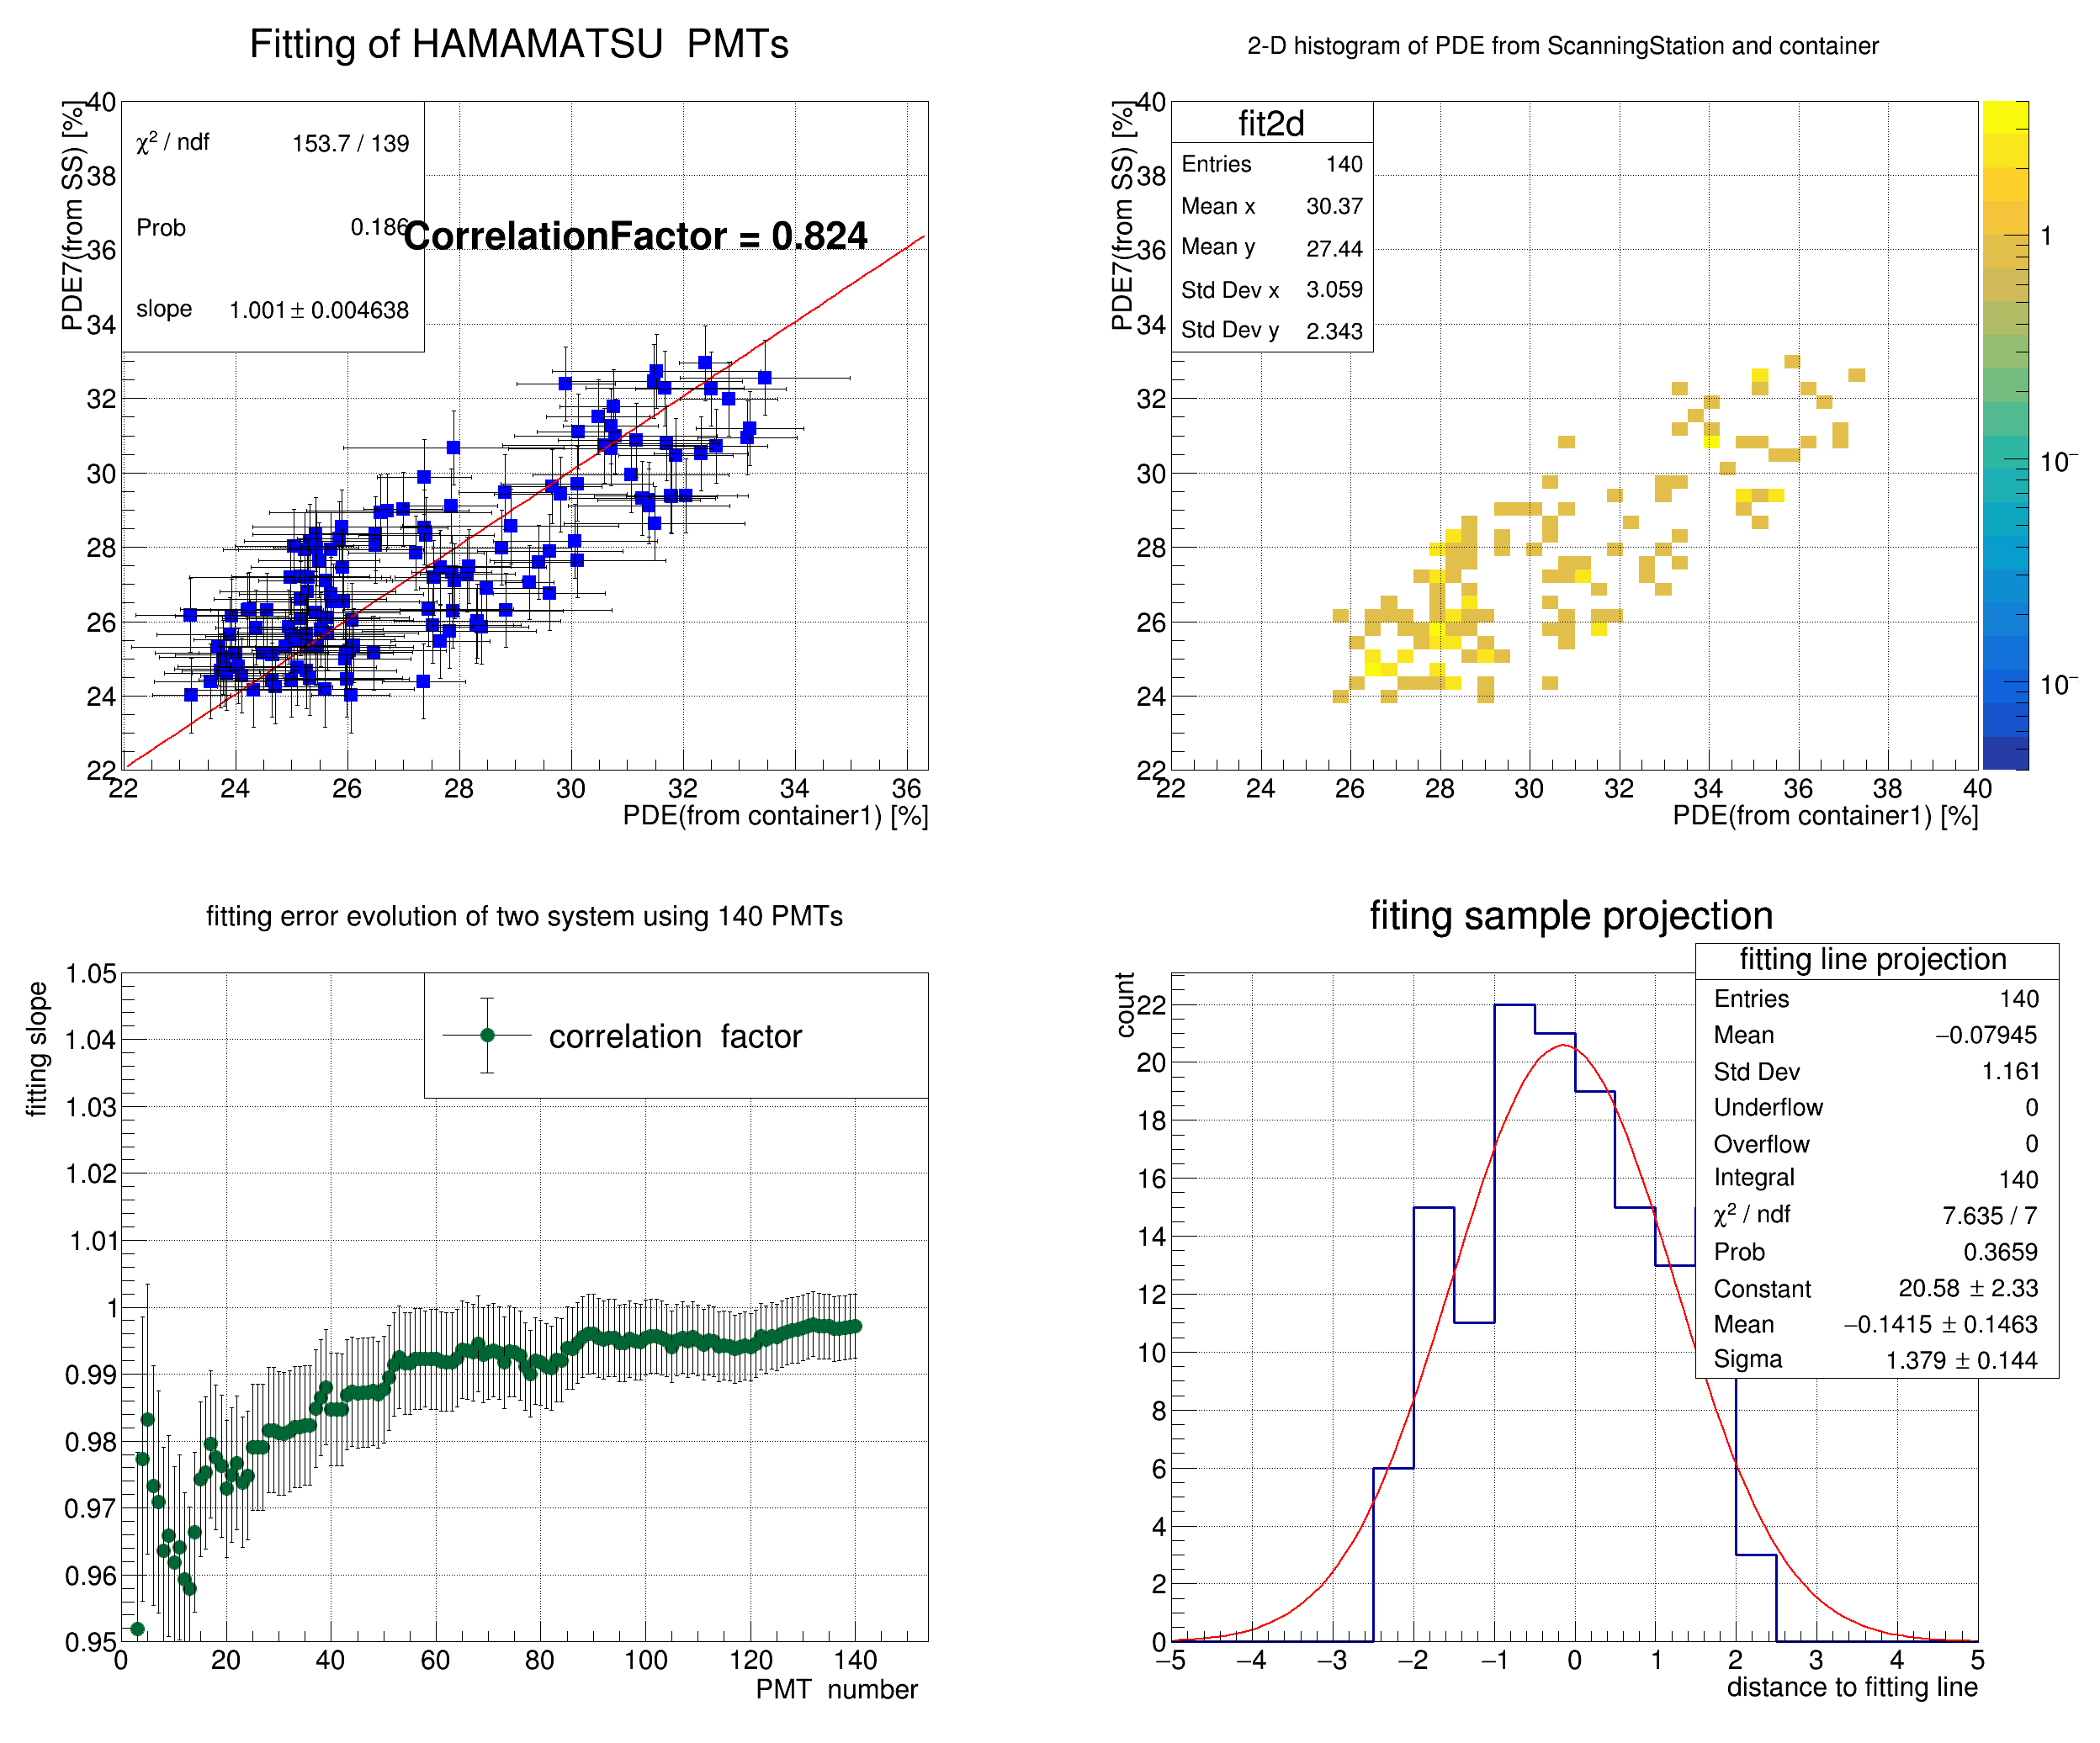
\includegraphics[width=0.58\textwidth]{fit_hmp_noint}
%\end{figure}
\end{frame}
%%%%%%%%%%%%%%%%%%%%%%%%%%%%%%%%%%%%%%%%%%%%%%%%%%%%%%%%%%%%%%%%%%%%
\begin{frame}{探测器性能模拟}
利用实验测量得到的塑闪的性能参数和光电器件的参数以及放射源刻度数据进行光学模拟。

基于GEANT4平台
\begin{itemize}
\item 探测器几何,闪烁体,PMT(SiPM),闪烁体界面
\item 物理过程(闪烁体的材料,衰减长度,光产额等参数)
\item 模拟不同的粒子源的响应($\gamma$,中子,正电子,$\mu$)
\item 能量响应
\item $\gamma,n$分辨能力
\end{itemize}
\end{frame}
%%%%%%%%%%%%%%%%%%%%%%%%%%%%%%%%%%%%%%%%%%%%%%%%%%%%%%%%%%%%%%%%%%%%
\begin{frame}{闪烁体发光时间测量}
\begin{figure}
\centering
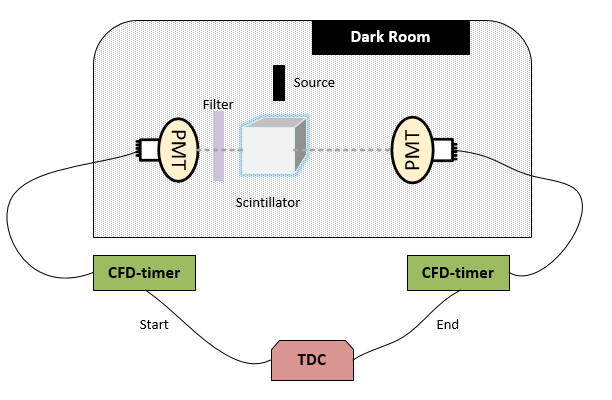
\includegraphics[width=.8\textwidth]{k_time} % 单图
\caption{闪烁体发光时间测量方案 }
\end{figure}

\end{frame}
%%%%%%%%%%%%%%%%%%%%%%%%%%%%%%%%%%%%%%%%%%%%%%%%%%%%%%%%%%%%%%%%%%%%
\begin{frame}{闪烁体光产额测量}
\begin{figure}
\centering
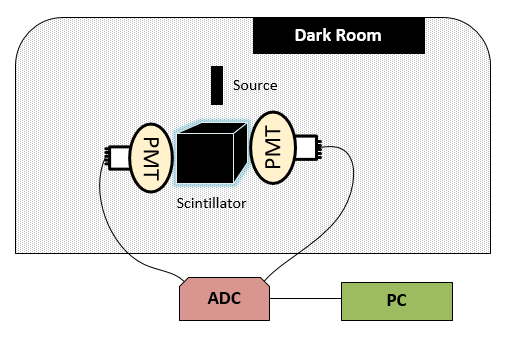
\includegraphics[width=.8\textwidth]{k_le} % 单图
\caption{闪烁体光产额测量方案 }
\end{figure}

\end{frame}
%%%%%%%%%%%%%%%%%%%%%%%%%%%%%%%%%%%%%%%%%%%%%%%%%%%%%%%%%%%%%%%%%%%%
\begin{frame}{闪烁体发光光谱测量}
\begin{figure}
\centering
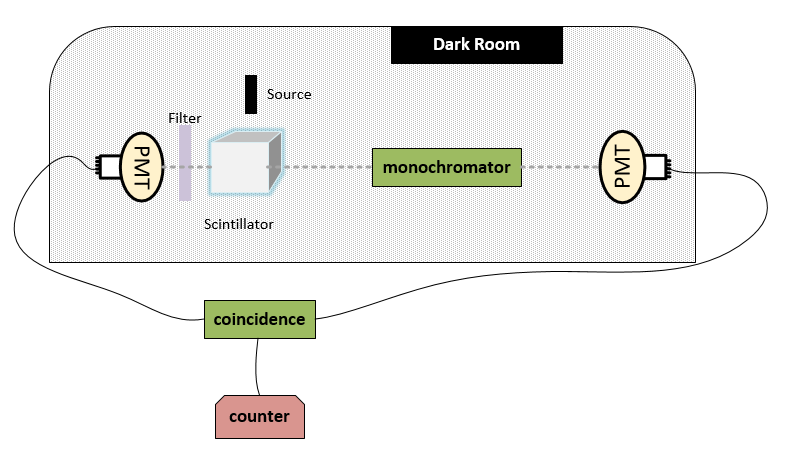
\includegraphics[width=.8\textwidth]{k_ls} % 单图
\caption{闪烁体发光光谱测量方案 }
\end{figure}

\end{frame}
%%%%%%%%%%%%%%%%%%%%%%%%%%%%%%%%%%%%%%%%%%%%%%%%%%%%%%%%%%%%%%%%%%%%
%\begin{frame}{数据分析}
%需要研究的问题
%\begin{itemize}
%\item 如何鉴别闪烁体的输出信号是$\gamma$还是中子产生的?
%\item 怎么样挑选中微子事例 
%\item $\mu$ veto 以及如何屏蔽环境本底
%\end{itemize}
%\end{frame}
%%%%%%%%%%%%%%%%%%%%%%%%%%%%%%%%%%%%%%%%%%%%%%%%%%%%%%%%%%%%%%%%%%%%
%\begin{frame}{硬件设施}
%\begin{figure}
%\centering
%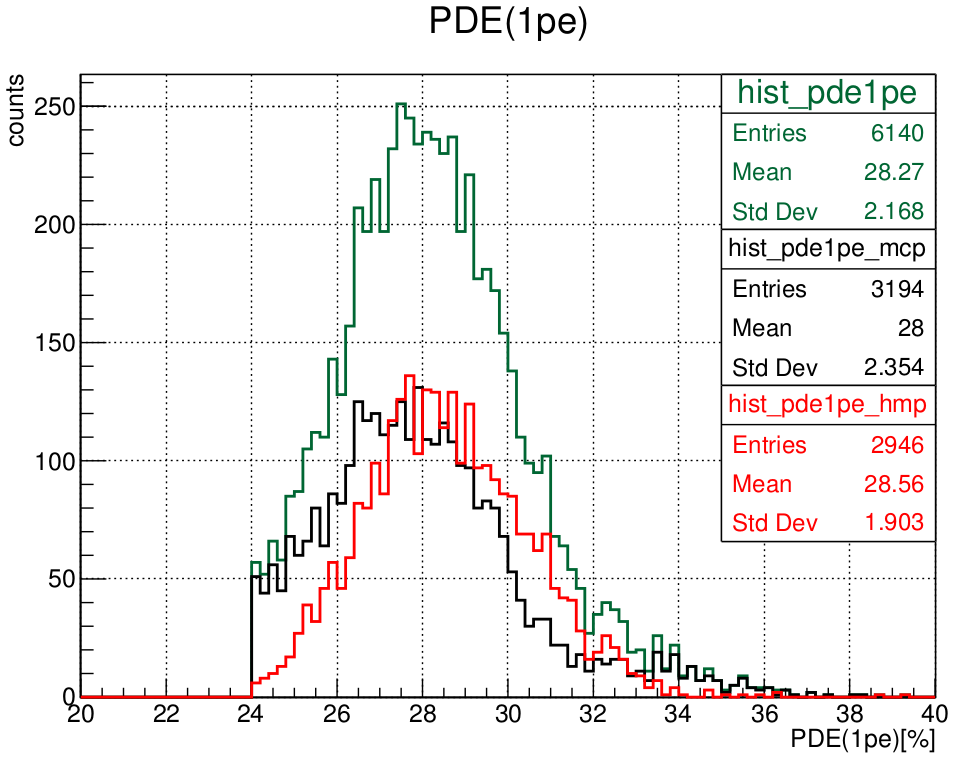
\includegraphics[width=0.45\textwidth]{pde_res}
%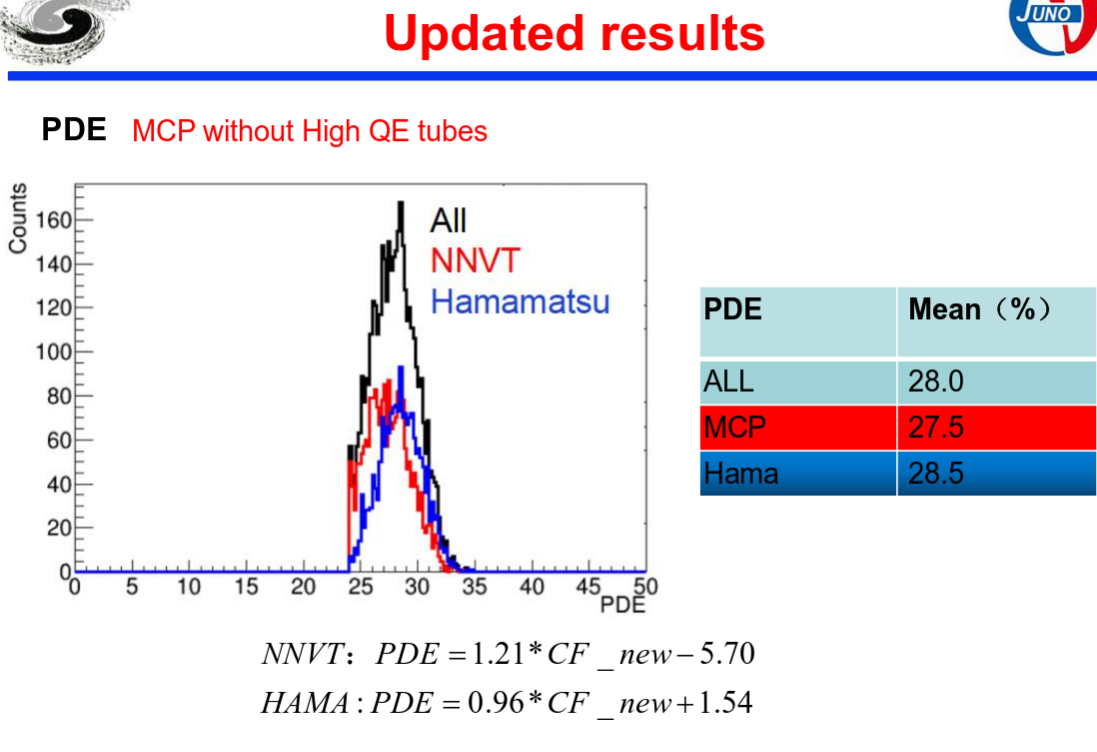
\includegraphics[width=0.45\textwidth]{hqpde}
%\caption{左图是抽屉累积拟合的结果,右图是现场所使用刻度方法结果\footnote{https://juno.ihep.ac.cn/cgi-bin/Dev\_DocDB/ShowDocument?docid=3646}}
%\end{figure}
%塑料闪烁体、PMT、高压模块、FADC、
%
%\end{frame}
%%%%%%%%%%%%%%%%%%%%%%%%%%%%%%%%%%%%%%%%%%%%%%%%%%%%%%%%%%%%%%%%%%%%
\section{已有工作和进度安排}
%%%%%%%%%%%%%%%%%%%%%%%%%%%%%%%%%%%%%%%%%%%%%%%%%%%%%%%%%%%%%%%%%%%%
\begin{frame}{schedule}
%\hrule{\textwidth}

\begin{columns}
\begin{column}{.5\textwidth}
现有基础:
\vspace{.5cm}
\hrule{\textwidth}
\vspace{.5cm}
\begin{itemize}
\item 中微子物理基础和JUNO相关的物理
\item JUNO 离线软件的使用和开发
\item JUNO PMT测试和数据分析经验
\item ROOT,GEANT4,C++,python 等软件 
\end{itemize}

\end{column}
\begin{column}{.5\textwidth}
时间进度:
\vspace{.5cm}
\hrule{\textwidth}
\vspace{.5cm}
\begin{itemize}
\item 研究塑料闪烁体的性能(18.11-19.03)
\item 探测器模拟和优化(18.11-19.06)
\item 参与近点探测器固体闪烁体原型搭建(19.06-19.11)
\item  近点探测器和JUNO主探测器关联的物理结果分析(---)
\end{itemize}
\end{column}
%\end{figure}
\end{columns}
\end{frame}
%%%%%%%%%%%%%%%%%%%%%%%%%%%%%%%%%%%%%%%%%%%%%%%%%%%%%%%%%%%%%%%
%%%%%%%%%%%%%%%%%%%%%%%%%%%%%%%%%%%%%%%%%%%%%%%%%%%%%%%%%%%%%%%
\section{总结}

\begin{frame}{总结}
\begin{itemize}
\item 精确测量反应堆中微子能谱对JUNO的物理目标很重要
\item  TAO的一种可能方案是使用固体闪烁体和PMT
\item  主要工作是探测器的模拟优化以及部分硬件搭建、调试 
\item  分析闪烁体的各种性能以及对中微子能谱的分辨能力
\end{itemize}
\end{frame}

\begin{frame}
\centering {\zihao{0} \color{red} \calligra{谢谢}}
\end{frame}


%\begin{frame}[allowframebreaks]
%\frametitle{References}
%\scriptsize
%\bibliographystyle{authordate1}
%\bibliography{R-GLMM-pkgs}
%\end{frame}

\appendix

\section*{附录}

%\begin{frame}{其他重要参数的check}
%HAMAMATSU-PMT的参数对比:
%
%\vspace{.5cm}
%
%\centering
%\begin{tabular}{l|c|c}
%\hline
%\hline
%参数(平均值)&  {\color{Blue} 我的结果} & {\color{Blue}测试现场结果} \\\hline
%暗计数(kHz)&17.8&16.6\\
%信号上升时间(ns)&7.3& 6.9\\
%信号下降时间(ns)&10.36& 10.2\\
%峰谷比&3.3& 3.9\\
%分辨率&0.28& 0.277\\
%高压(V)&1861& 1858\\
%信号半高宽(ns)&9.08& 11.6\\
%\hline
%\end{tabular}

%\begin{table}[htbp]  
%\caption{PMT typical performance}  
%\resizebox{.8\textwidth}{!}{%
%\begin{tabular*}{.98\textwidth}{l|cccc}
%%\toprule  
%\hline  
%\hline  
%Performance & PDE &DCR & TTS& uniformity \\  
%\hline  
%HAMAMATSU &  lower\% & 20 kHz& 3ns& worse \\  
%NNVT  & higher\% & 40kHz & 7ns& better \\  
%\hline  
%\end{tabular*}  
%%}
%\end{table} 

%\end{frame}
%\begin{frame}{其他重要参数的check}
%MCP-PMT的参数对比:
%
%\vspace{.5cm}
%
%\centering
%\begin{tabular}{l|c|c}
%\hline
%\hline
%参数(平均值)&  {\color{Blue} 我的结果} & {\color{Blue}测试现场结果} \\\hline
%暗计数(kHz)&41.4&44.3\\
%信号上升时间(ns)&3.2& 4.6\\
%信号下降时间(ns)&15.9& 16.2\\
%峰谷比&3.19& 4.4\\
%分辨率&0.35& 0.32\\
%高压(V)&1783& 1784\\
%信号半高宽(ns)&5.8& 7.7\\
%\hline
%\end{tabular}
%\end{frame}
%%%%%%%%%%%%%%%%%%%%%%%%%%%%%%%%%%%%%%%%%
%%%%%%%%%%%%%%%%%%%%%%%%%%%%%%%%%%%%%%%%%%%
%\begin{frame}{平均PDE}
%每个抽屉的平均PDE分布:
%\begin{figure}
%\centering
%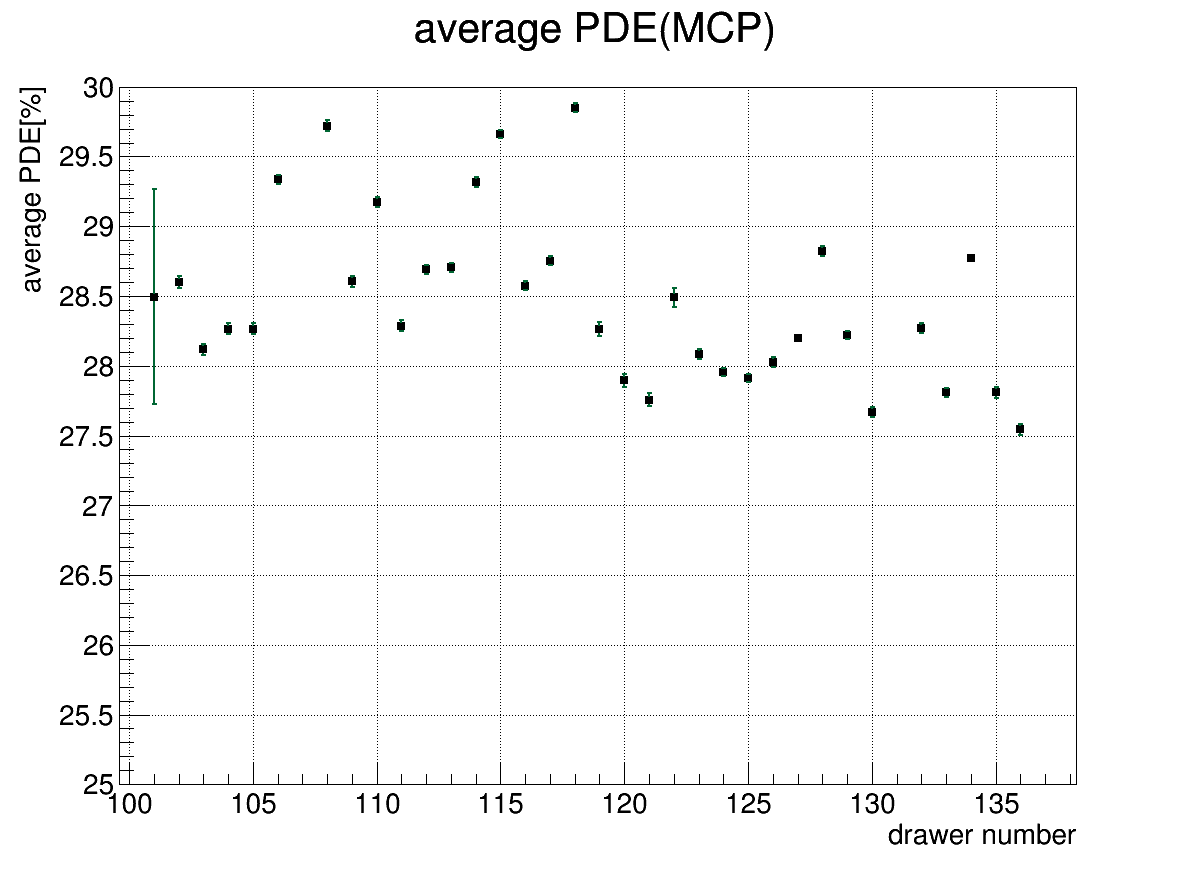
\includegraphics[width=0.88\textwidth]{dpde}
%\end{figure}
%\end{frame}
%% OpenBUGS  WinBUGS  JAGS
% library(R2OpenBUGS) # 2017-2-20 version 3.2-3.2
% library(R2WinBUGS) # 2015-07-29 version 2.1-21
% library(rjags) # 2016-02-19 version 4-6
% library(BRugs) # OpenBUGS 2017-06-26  version 0.9-0
% library(glmmBUGS) # Generalised Linear Mixed Models with BUGS and JAGS 2016-09-22 version 2.4.0
% library(R2jags) # Using R to Run 'JAGS'  2015-08-23	 version 0.5-7

% network
	% diagram DiagrammeR DiagrammeRsvg
 % library(help=graph)

 % library(help=Rgraphviz)
 % library(help=igraph)


%\begin{frame}{Ack}
%\begin{itemize}
%\item[\faGithub] \href{https://github.com/Cloud2016}{Cloud2016} \faAt Github
%\item[\aiOverleaf] \href{https://www.overleaf.com/}{Xiangyun} \faAt Overleaf
%\item[\aiarXiv] \href{https://arxiv.org/}{arXiv}
%\end{itemize}
%\end{frame}

\end{document} 


